\documentclass[acmsmall]{acmart}

\usepackage{pdfpages}
\begin{document}

\title[Towards user-friendliness in theorem provers]{Towards user-friendliness
  in proof assistants: an effect-based attempt}

\author{April Gonçalves}
\email{april@cyberglot.me}
\affiliation{
  \institution{Metastate AG}
  \city{Edinburgh}
  \state{UK}
}

\renewcommand{\shortauthors}{April Gonçalves}

\begin{abstract}
Proof assistants provide a framework for modelling and verification of
theories, as well as trust-worthy software. However, such power is usually only
available to experts. We propose a new approach, based on algebraic effects and
handlers, to integrate different automated proof strategies that enables
newcomers to take advantage of proof assistants without a more in-depth
understanding of underlying theory. Our approach gives beginner users an effect
system, a handful of effectful strategies (tactics, proof search and a SMT
solver) and their handlers under a shared interface, while advanced users can
extend our system with new effects and new handlers. Lastly, we prototype the
system as a library in Agda. While our prototype is minimal, it shows how easily
proofs can be carried on so long as the user has the correct intuition. We
believe our system empowers non-experts and has the potential to bring verified
software to many relevant industries, such as finance.
\end{abstract}

\keywords{effect handlers, proof assistants, user experience}

\maketitle

\section{Verification for the Masses}

The usability of proof assistants such as Coq, Agda, Isabelle/HOL and Twelf is
hard to measure: all of them require significant domain knowledge that
frequently matches a deeper understanding of Type Theory, the theory that
enables such assistants to exist. Coq and Isabelle/HOL are more commonly applied
outside their niche, and their programming style is sharply different from
mainstream programming and even functional programming. Granted, they come with
their own integrated development environment (IDE), which may make it easier for
students and newcomers. To our knowledge, no usability study has been
held for a proof assistant, however there exists studies that account for
an informal ``usability'' criteria -- they appear to measure how fast users can
familiarise themselves with the system or IDE.

Folklore within the proof assistants community seems to show that typical users
find Coq hard to use due to a large library of tactics and difficult readability
of the code after its completion. Many Coq learning materials suggest users to
add comments for structural induction cases and inductive hypothesis. As
mentioned, no user studies were conducted to attest such hypotheses.

It also has to be granted that proof assistants are relatively new technology
and there are no guidelines or even an intuition on how such systems should
perform or what features should be available to the users. The closest model we
have are proofs by hand, however, following that model for proof assistants has
two main pitfalls: (a) proofs by hand are also not widely taught in mathematics
classes during school years; and (b) proofs by hand and automated proof
writing employ fundamentally different paradigms, where the latter requires
axioms and formulations to be encoded explicitly, commonly known as a ``pedantic
proof style''.

\subsection{Empowering users of different levels of expertise}

To popularise software verification, we mush make proof writing less of a
burden to the user. Currently, only specialists can write proofs for their
programs, even though the working programmer understands the domain and
invariants of their projects -- otherwise they would not be able to write any
software. \textit{Our hypothesis is that programmers are well-equipped to derive and
prove properties of their software, but they lack the mathematical maturity and
vocabulary to carry on a formal proof. } We have evidence that students fail to
produce well-made proofs due to the lack of mathematical maturity, even though
they do understand the subject matter at hand.

In our approach, we propose an (algebraic) effects and handlers view of such
proofs, based on prior work developed by the Andromeda proof assistant. Here,
our users will program as they would normally and invoke
a proof environment as an effect to prove certain properties as they go. Given
that the proof environment is \textit{just} an effect, we envision that different proof
styles (e.g, Agda-style dependent types, SMT solver, proof search) can be ``composed''
under a shared interface, a proof object that can manipulate itself while
querying different automated proof engines.

The reasons we employ algebraic effects and handlers are manifold:
\begin{enumerate}
\item as proofs cannot be fully automated, all approaches that try to automate
  the process (e.g, proof search, SMT solver) may either be non-deterministic or
  never find a solution. Therefore, the system should be able to handle
  ``impure'' computations and errors. Algebraic effects and handlers have
  well-defined semantics and provide a simple interface for performing effects.
  With them, we avoid indiscriminate effects that are often error-prone and
  intricate effects machinery such as monad transformers;
\item its semantics accommodate composition of arbitrary effects and the
  composition of multiple handlers, which means users have the ability to weaken
  more general strategies into specific ones while maintaining the original untouched;
\item it has well-defined semantics, and it is the main feature of many new
  research languages, such as Koka, Eff, Frank and Effekt, what suggests a greater
  potential to be investigated further.
\end{enumerate}

\subsection{Goals and Contributions}

The present project is still under development, and we intend to develop a core calculus and a
full compiler-level implementation into the Juvix\footnote{Juvix is a
  dependently-typed programming language for smart contracts. More information
  at juvix.org} programming language.

\paragraph{Goals} The project exists to enable users to write safe, verified
code without investing time into learning dependent types and theorem proving.
The project's goals are presented as follows:
\begin{enumerate}
\item make software verification more accessible to programmers familiar with
  functional programming;
\item foster knowledge sharing between domain experts and regular programmers;
\item lower the barrier to entrance into software verification to non-experts.
\end{enumerate}

\paragraph{Contributions} While the project is a work-in-progress, this paper
provides three important contributions that lays out the full extent of the
work, which are presented as follows:
\begin{enumerate}
\item a specification of a user interface for automated proofs based on
  algebraic effects and handlers that permits user-defined effects for proof
  strategies, and also user-defined handlers for existing effects (Section \ref{intro-witch});
\item a minimal prototype in Agda that validates the feasibility of such system
  (Section \ref{witch-agda});
\item a short technical account of the effort required to materialise such a
  user interface into proof assistants (Section \ref{tech-details}).
\end{enumerate}

\section{Introducing Witch} \label{intro-witch}

\begin{figure}[!ht]
   \centering
    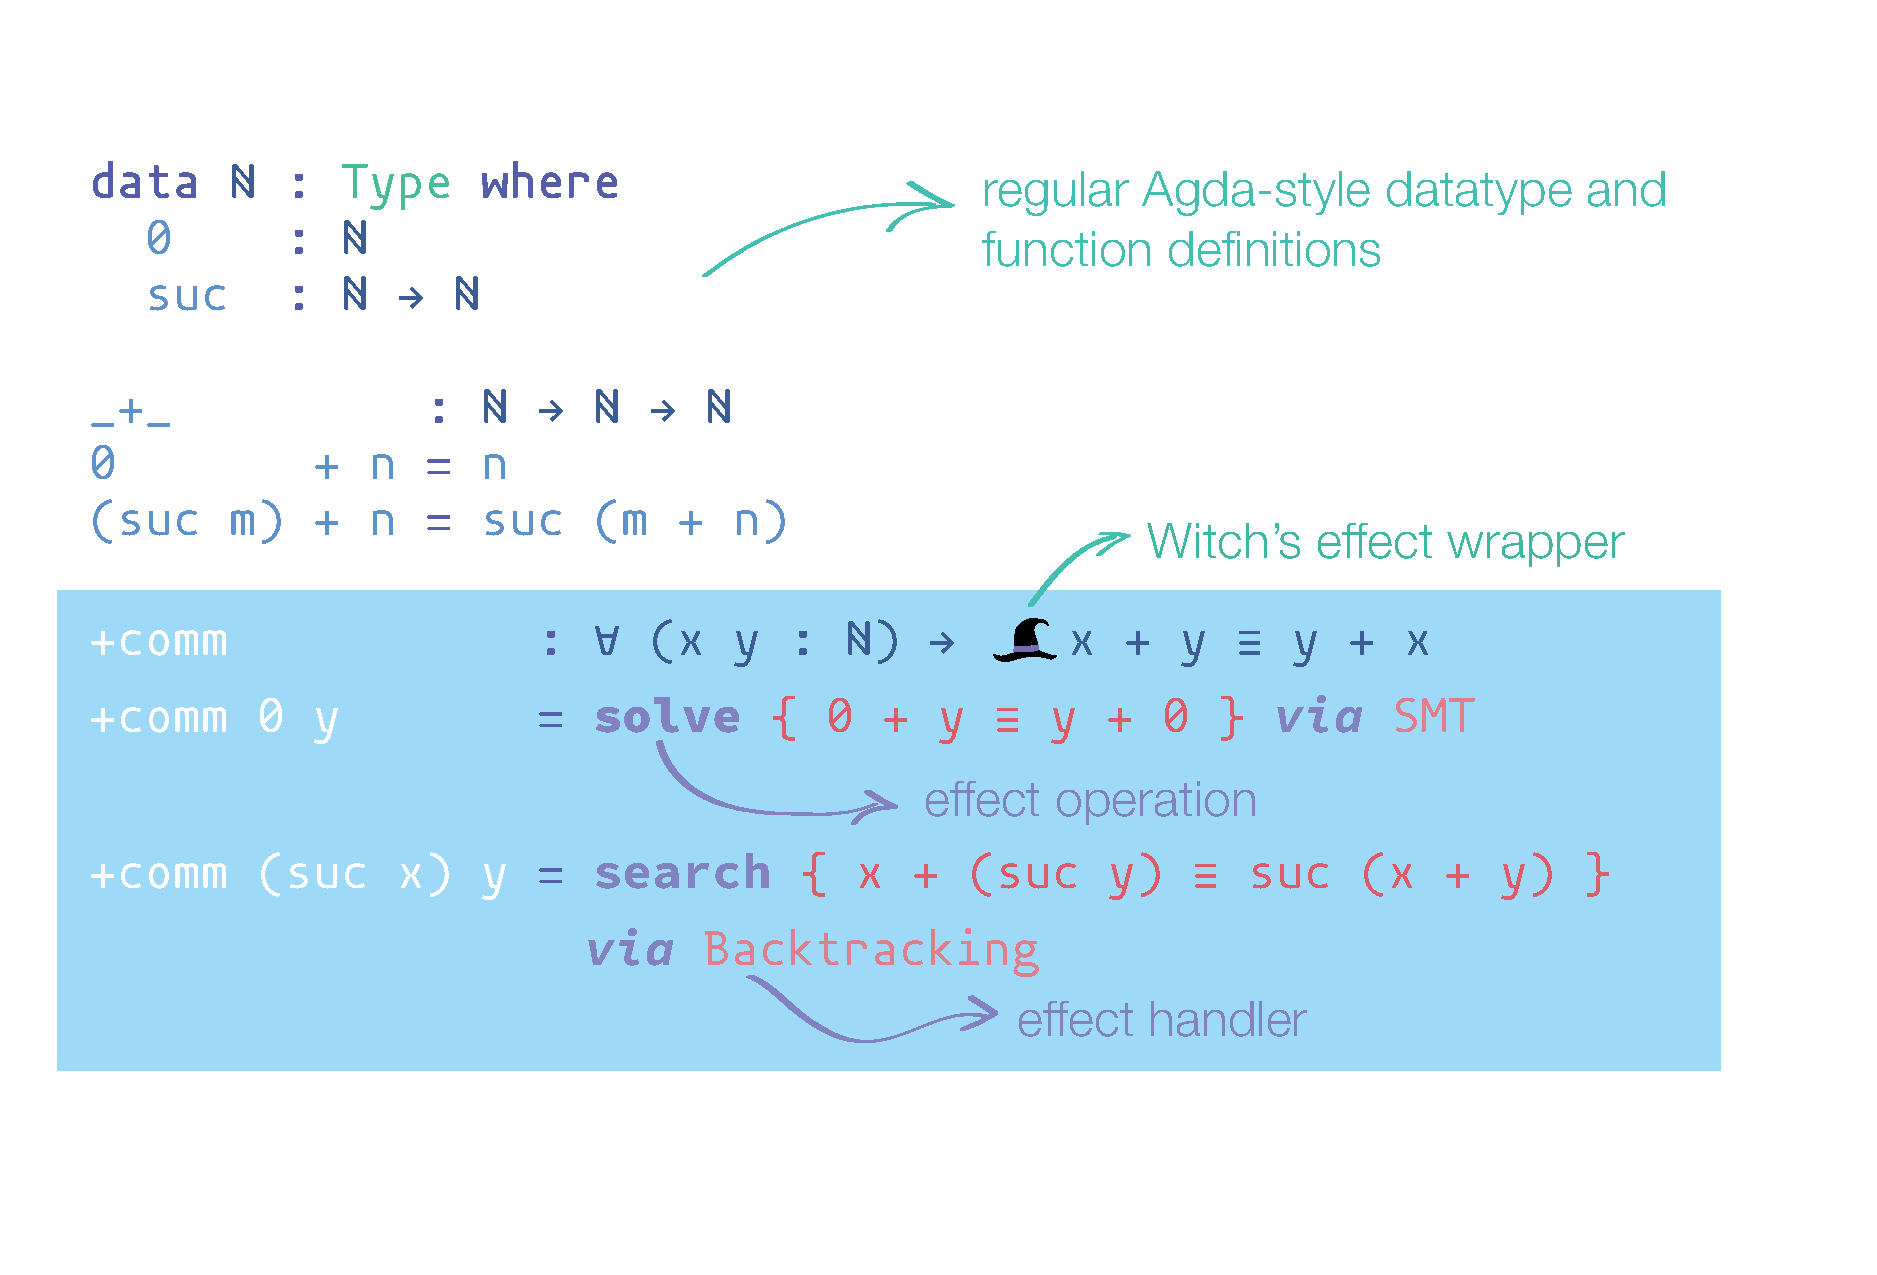
\includegraphics[width=\textwidth]{image/witch.eps}
    \caption{Low-fidelity prototype of Witch}
    \label{fig:prototype}
\end{figure}

In this section, we introduce our tool, named Witch.

\paragraph{Downsides of our approach}
There are two main styles for writing proofs within a proof assistant: external
verification and internal verification. The latter concerns itself with code
that is \textit{correct-by-construction}, meaning that only valid states allowed and it
carries all information necessary to make proofs trivial; while the former
concerns itself with proofs about non-proof-carrying code.
Witch's primarily focus is on external verification. We believe that newcomers
will struggle to write proof-aware code, since it departs strongly from
mainstream programming, even within the functional style. We expect users to
write their code as they normally would do and then prove necessary properties.
However, Witch does not support writing correct-by-construction code.

\section{Witch in Agda} \label{witch-agda}





\paragraph{Why Agda?} Agda provides high-level meta-programming constructs, and
its coding style is a reminiscent of ML family of functional programming languages.

\subsection{Technical Effort Required} \label{tech-details}

Although Witch is implementable at the library level, it requires that proof
assistants to provide a set of off-the-shelf features. The most important
feature is type-level meta-programming. Witch is only possible given the proof
assistant's ability to manipulate its own proof terms to generate new variables,
holes, goals, among others and manipulate terms and types in a proof-carrying
fashion. Secondly, the proof assistant should feature an interface with the
outside world. Although it is not inherently a requirement, its absence means
that no solver will be integrated, diminishing the proposed value of the tool.
Lastly, proof assistants must support algebraic effects and handlers. If there
is no built-in solution, a library-level solution is possible -- as we did in
Agda. However, a solid implementation may not be trivial to achieve. In Agda,
we translate all calls into optimised continuation-passing style that inlines
all calls. This strategy also works at compiler-level if necessary. There are
many strategies to efficiently implement algebraic effects and handlers, but we
went for the one that seemed the most straight-forward method to implement it in Agda.

\end{document}
\endinput
